\begin{frame}{Evolución de reservas \small{(compromisos del año anterior pendientes por obligar)}}
\begin{figure}[h!]
\centering
%\caption{Evolución de reservas (compromisos del año anterior pendientes por obligar)}
\label{fig:reservas}
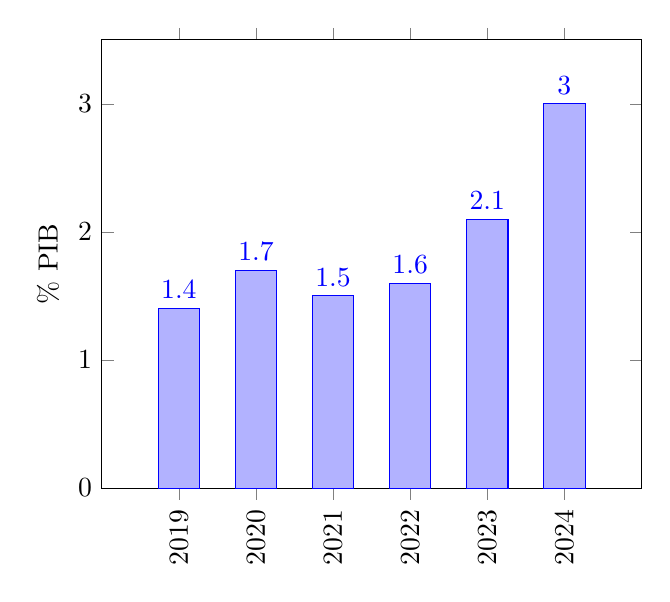
\begin{tikzpicture}
    \begin{axis}[
        ybar,
        symbolic x coords={2019, 2020, 2021, 2022, 2023, 2024},
        xtick=data,
        xticklabel style={rotate=90, anchor=east},
        ylabel={\% PIB},
        ymin=0, ymax=3.5,
        bar width=15pt,
        nodes near coords,
        enlarge x limits=0.2
    ]
        \addplot coordinates {
            (2019,1.4)
            (2020,1.7)
            (2021,1.5)
            (2022,1.6)
            (2023,2.1)
            (2024,3.0)
        };
    \end{axis}
\end{tikzpicture}
\vspace{0.1cm}
%\par\footnotesize{\textit{Fuente: Elaboración propia con base en ejecución presupuestal del rezago con recursos de la Nación excluyendo deuda a enero de cada año, Ministerio de Hacienda.}}
\end{figure}
\end{frame}
